\chapter{A Two-Fold Framework for AIBOM in Cognitive Workflows}\label{ch:chapter2}


This chapter presents our proposed methodology for incorporating SBOM-driven approaches (extended to the AIBOM scope) within a multi-agent cognitive workflow. The chapter is structured as follows: Section~\ref{sec:proposal} outlines the conceptual design and meta-level orchestration strategies that form the foundation of our approach; Section~\ref{sec:AIBOM-system-of-agents} introduces the SALLMA architecture, a multi-agent system whose principles are employed in our proposal; finally, Section~\ref{sec:design-and-implementation} details the design and implementation of the proposed system, providing concrete examples of how the theoretical framework translates into a working solution. 

Supporting materials, including comprehensive UML diagrams and our testing strategy, are provided in Appendix~\ref{appendix_details}.


\section{Our Proposal} \label{sec:proposal}

This study proposes a two-fold framework designed to address the critical gaps previously identified in the literature (see Section \ref{sec:gaps}). It specifically targets the persistent challenges of reliability, structural adaptability, and comprehensive traceability within AI-driven multi-agent systems. The framework comprises two distinct aspects that together underpin the proposed approach.

The first aspect involves a dedicated design pattern adapted from the Reflection Architectural Pattern (see Section \ref{sec:reflection}), tailored for agent-based systems. This pattern, defined as a means of "changing the structure and behavior of software systems dynamically" \cite{Buschmann1996}—is used to enable self-awareness and run-time adaptability.

The second aspect addresses traceability by extending standard Software Bill of Materials (SBOM) practices to include AI-specific artifacts, thereby formalizing the Artificial Intelligence Bill of Materials (AIBOM). The AIBOM provides a structured record of models, datasets, hyperparameters, prompts, tools, and agent configurations, supporting transparency and accountability across the AI system lifecycle.



\subsection{The Reflection Architectural Pattern}
\label{sec:reflection}

We argue that leveraging the Reflection Pattern offers clear benefits for the AIBOM. To support this claim, we first provide an overview of the pattern and its key mechanisms.

The Reflection architectural pattern enables software systems to dynamically adapt their structure and behavior at runtime. As described by Buschmann et al.~\cite{Buschmann1996}, it achieves this by dividing the system into two levels: a \textbf{meta-level}, which holds \textit{metaobjects} encapsulating information about system properties (such as type structures or communication mechanisms), and a \textbf{base level}, which implements the core application logic. The key idea is that changes to metaobjects, via a well-defined \textbf{metaobject protocol} (MOP) that ensures consistent modifications, directly influence the behavior of the base level without altering its source code. Consequently, the implementation of the base level uses the meta-objects to remain independent of all aspects prone to alteration.

An overview of the general structure of a reflective architecture is illustrated in Figure~\ref{fig:reflection}, which highlights the layered interaction. This separation supports system evolution, flexibility, and the ability to respond to changing requirements. 

\begin{figure}[h]
    \centering
    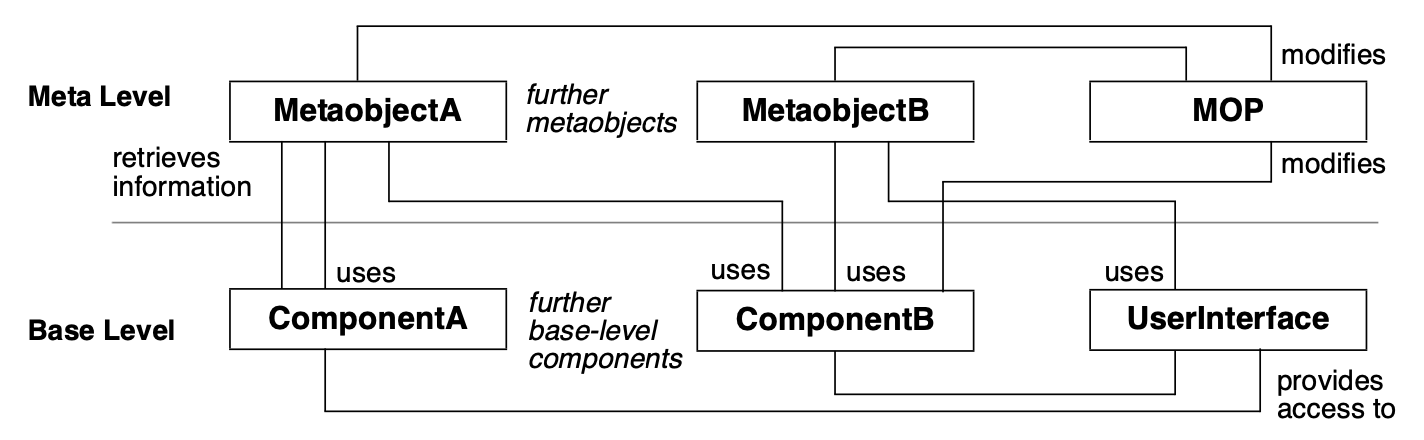
\includegraphics[width=1\textwidth]{Template_tesi/img/reflection.png}
    \caption{Architectural overview of a reflective system, illustrating the meta and base levels and their interactions. From \textit{Pattern-Oriented Software Architecture}, Buschmann et al.~\cite{Buschmann1996}.}
    \label{fig:reflection}
\end{figure}

In the context of this study, the presented pattern is fundamental as it allows for the dynamic management of a \textit{repository of meta-models}, without the need to define in advance the components with which the agents or the system will interact. As a result, agent interactions are dynamically modeled, leading to a structured cognitive workflow. In summary, a reflective approach yields the following key benefits:

\begin{itemize}[leftmargin=*, label=--] 

\item \textbf{Dynamic reconfiguration}: The system can adapt its behavior and structure at runtime based on changes to its meta-level, without requiring redeployment. 

\item \textbf{Separation of concerns}: By decoupling the application logic (Base Level) from the Knowledge Layer (Meta Level)—which is subject to more frequent changes—maintainability and extensibility are significantly improved.

\item \textbf{Semantic interoperability}: Components with no prior knowledge of each other can interact seamlessly. This enables the integration of heterogeneous agents into cohesive workflows, allowing the composition of complex and adaptive interactions.

\item \textbf{Explainability and traceability}: By observing the system’s components and behaviors, the meta-level establishes a foundation for a self-aware and auditable architecture. This allows the system to track its composition, explain the rationale for the decision, and trace the results.

\end{itemize}




\subsection{Integration of the Two-Fold Framework}


The novel and primary contribution of this work lies in integrating the Reflection Pattern, which provides structure and adaptability, with the AIBOM formalism, which ensures traceability. By coupling the comprehensive AIBOM inventory with the Reflection pattern, each cognitive workflow gains visibility into:

\begin{itemize}[leftmargin=*, label=--]
    \item \textbf{Its own structural elements} --- including agent composition, model versions, training data references, and external libraries.
    \item \textbf{Its meta-level} --- a supervisory layer that monitors changes, performs reconfiguration, and enforces security or compliance rules.
    \item \textbf{Runtime adaptations} --- triggered by environment changes, updates to agent dependencies, or new user requirements, all logged and documented within the AIBOM to maintain continuous traceability.
\end{itemize}

\noindent
This integration of reflection and AIBOM serves as the foundation for a self-aware and self-adapting multi-agent system. The architecture we propose includes:


\begin{itemize}[leftmargin=*, label=--]
    \item \textbf{Core AI Agents}: Responsible for distinct tasks (e.g., user intent detection, route planning, resource allocation).
    \item \textbf{Meta-Level Controller}: Dynamically adjusts agent configurations by referencing the AIBOM, ensuring only approved/compatible components are used.
    \item \textbf{AIBOM Repository}: Storing SBOM-like records for each AI component and its lifecycle events.
\end{itemize}

\noindent
By adopting this layered approach, we aim to demonstrate how cognitive workflows can be more traceable, transparent, and compliant with emerging AI regulations, especially where multi-agent collaboration requires detailed knowledge of each component’s provenance and behavioral characteristics.


\section{LLM-based System of Agents} 
\label{sec:AIBOM-system-of-agents}

AIBOM can be a valuable tool for managing complex systems composed of LLM agents by introducing the level of transparency and traceability typically associated with Software Bills of Materials. As foundation models rapidly transform the methodologies used to develop and deploy software-intensive systems, emerging approaches must embrace this shift by adopting novel architectural designs that address distributed, real-world scenarios rather than relying on conventional centralized solutions. In this context, the present study builds upon the work of Becattini, Verdecchia, and Vicario at the Software Technologies Laboratory, University of Florence \cite{becattini2025sallma}, extending their proposed \textbf{SALLMA} architecture.


\subsection{SALLMA Architecture Overview}
\label{sec:sallma}


\begin{figure}[h] 
    \centering
    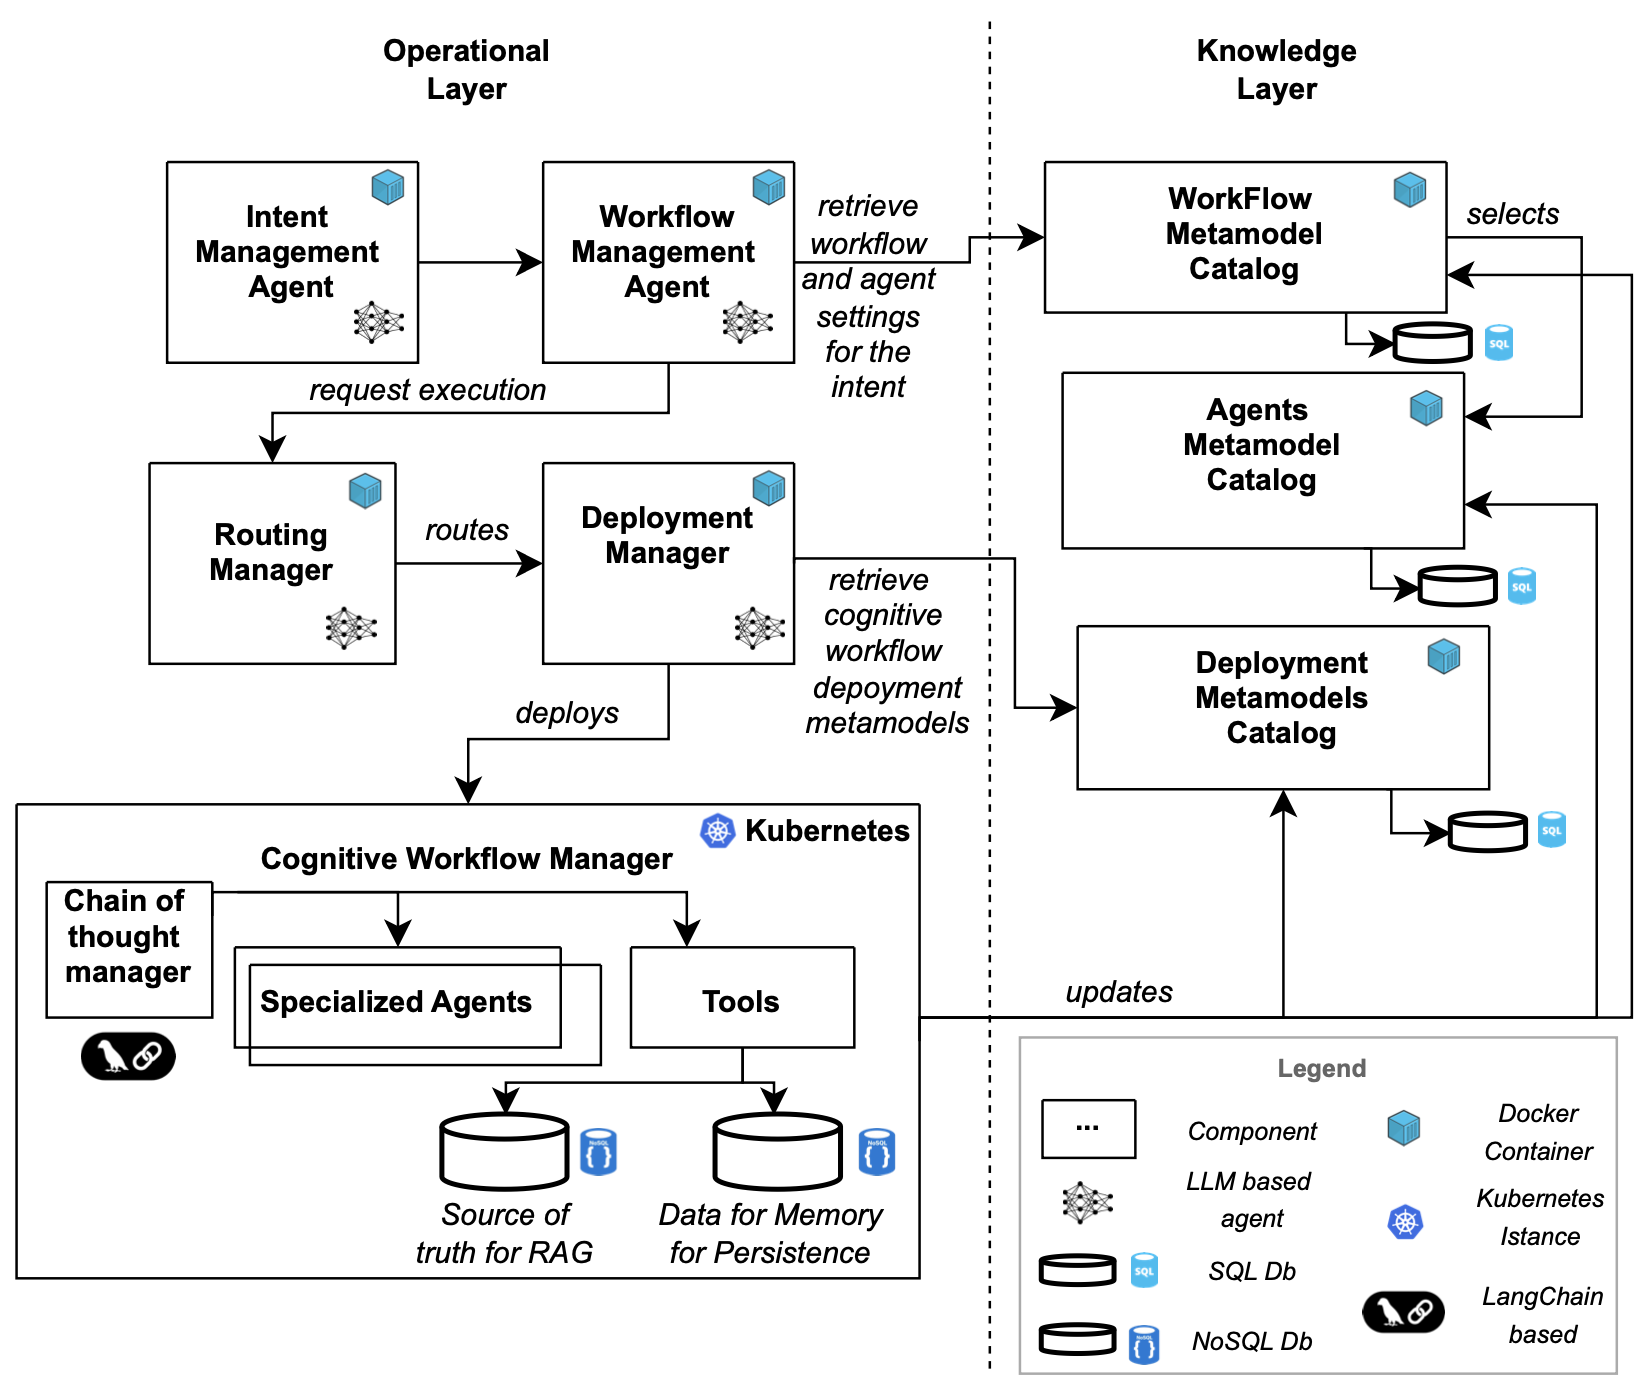
\includegraphics[width=.9\textwidth]{Template_tesi/img/SALLMA.png}
    \caption{SALLMA Architecture Overview}
    \label{fig:SALLMA}
\end{figure}
An introduction to the concept of SALLMA (Software Architecture for LLM-Based Multi-Agent Systems) will first be provided.
SALLMA  is a distributed, multi-agent architecture featuring an Operational Layer for real-time task execution and a Knowledge Layer for workflow and agent configuration meta-model management. Engineered from first principles, it is inherently modular and adaptive, designed to orchestrate multiple large language model (LLM) agents across both cloud and edge environments. While primarily a conceptual architecture, a proof of concept has been implemented to evaluate its functional suitability. 


By introducing a dual-layer structure, SALLMA addresses the limitations inherent in single-agent LLM systems, enabling dynamic adaptability of the system to the diversity of tasks in real-world applications. Notable limitations commonly observed in single-agent approaches include:

\begin{itemize}[leftmargin=*, label=--]
    \item Suboptimal hyperparameter configurations for specific requests.
    \item Lack of persistent memory.
    \item Limited access to ground-truth data.
    \item Challenges in reliability and sustainability management.
\end{itemize}

Compared to a single monolithic AI agent, an ensemble of specialized agents enables dynamic task decomposition and organic specialization: each agent can focus on its strengths, and tasks can be distributed dynamically across the system. Furthermore, this approach introduces fault tolerance: if one agent fails, others can continue execution, resulting in greater robustness and reliability.

A comprehensive overview of the SALLMA architecture is illustrated in Figure~\ref{fig:SALLMA}, highlighting the distinction between its two core layers. A brief explanation of each layer follows.

\subsubsection{SALLMA Operational Layer}

The Operational Layer acts as the dynamic core that is responsible for handling real-time interactions and orchestrating task-specific agents. Essentially, it is where the LLM agents “live” and interact, and is thus responsible for the decision-making process of the workflow. The primary elements of the Operational Layer are:

\begin{itemize}[leftmargin=*, label=--]
    \item\textbf{Intent Management Agent}: Parses the request and sets up the system to retrieve workflows using predefined intents stored in the Knowledge Layer.
    \item\textbf{Workflow Management Agent}: Breaks tasks into subtasks, assigning them to specialized agents.
    \item\textbf{Routing Manager}: Determines whether an existing workflow instance can handle the request or a new instance is required.
    \item\textbf{Deployment Manager}: Deploys workflows by leveraging the configurations and resources outlined in the Knowledge Layer.
    \item\textbf{Cognitive Workflow Manager}: Orchestrates tasks within a containerized environment, leveraging specialized agents, a chain-of-thought process, persistent memory for context-aware execution, and foundational data for reliable retrieval-augmented generation (RAG).
\end{itemize}





\subsubsection{SALLMA Knowledge Layer}
The Knowledge Layer is dedicated to storing and managing information that agents use or produce. It serves as the foundation for SALLMA's meta-model management, maintaining an inventory of reusable workflows and agent configurations. Agents in the Operational Layer rely on the Knowledge Layer both to retrieve relevant data and to update it with new findings or changes in state. Among its components, the most notable include:

\begin{itemize}[leftmargin=*, label=--]
    \item\textbf{Workflow Metamodel Catalog}: Stores predefined workflow configurations optimized for different tasks.
    
    \item\textbf{LLM Configuration Catalog}:  Contains predefined configurations for each LLM agent (e.g., hyperparameters, resource allocations, and so on).

    \item\textbf{Deployment Metamodels Catalog}: Holds a set of deployment models that detail the proper cognitive workflow configurations for each operational scenario (e.g., cloud or edge environments).
\end{itemize}






\subsection{Extending SALLMA}
\label{sec:ext-sallma}


The proposed framework integrates SBOM management into the SALLMA multi-agent system architecture. By extending SALLMA, we introduce a systematic way to document and track the composition of each agent within the Knowledge Layer and to use that data in the Operations Layer for better decision-making and security inspections. In contrast to traditional practices that rely on the static generation of SBOMs and their passive use for tracking dependencies, this novel approach marks a paradigm shift toward dynamically leveraging SBOM knowledge within the system across its entire lifecycle. The key idea is that as the multi-agent system evolves, it will generate and maintain an SBOM that describes all its software components (agents, models, libraries, and dependencies); this self-describing inventory of components information will be actively used by the system for governance and maintenance, enhancing trust in what the AI is executing.

A limitation of the approach outlined in SALLMA is the lack of a clear formalization regarding information ownership, specifically whether it should reside within the Knowledge Layer or be delegated to external systems and accessed via retrieval augmented generation (RAG).
In this context, an AIBOM approach could be beneficial, as it allows a more proper and elegant differentiation between the knowledge layer—where meta-models of the cognitive workflows are stored—and the data level, where data belongs.






\section{System's Design and Implementation}\label{sec:design-and-implementation}

The following section details the architecture and core components of the proposed system in its design and final implementation. Building on the conceptual foundations introduced earlier, it outlines the structural patterns, persistence strategies, execution mechanisms, and dynamic adaptation features that enable the orchestration of cognitive workflows. Every design choice is motivated by the need for extensibility, modularity, and runtime flexibility in managing AI agents and their meta-structures. The demonstration implementation is carried out in Java, leveraging the emerging Spring AI framework from the Spring ecosystem to support AI engineering tasks (see Appendix \ref{ch:appendix_spring} for a detailed explanation of this choice). As a proof of concept, although SALLMA was conceived as a distributed architecture, the concrete implementation proposed to support the study is based on a single application where workflow nodes are instantiated in memory rather than deployed as separate services. This simplification maintains the core concepts while allowing for comprehensive validation of the system's logic and interaction patterns.






\subsection{Pattern Outline}


As previously introduced, the proposed architecture adheres to the SALLMA philosophy, adopting a dual-layered structure comprising the Knowledge Layer and the Operational Layer. Leveraging the Reflection Pattern alongside aggregation and subclassing, the architecture achieves a high degree of flexibility.
The Operational Layer hosts the execution-time entities: instance nodes and workflows; each instance is linked to a corresponding meta-model, which belongs to the Knowledge Layer and governs its actual runtime behavior. Across both layers, as illustrated in Figure \ref{fig:nodes-reflection-uml}, specialized nodes encapsulate different AI models and external tools (e.g., LLMs, Embedding Models, RESTful Services, Vector Databases, etc.).

\begin{figure}[h]
    \centering
    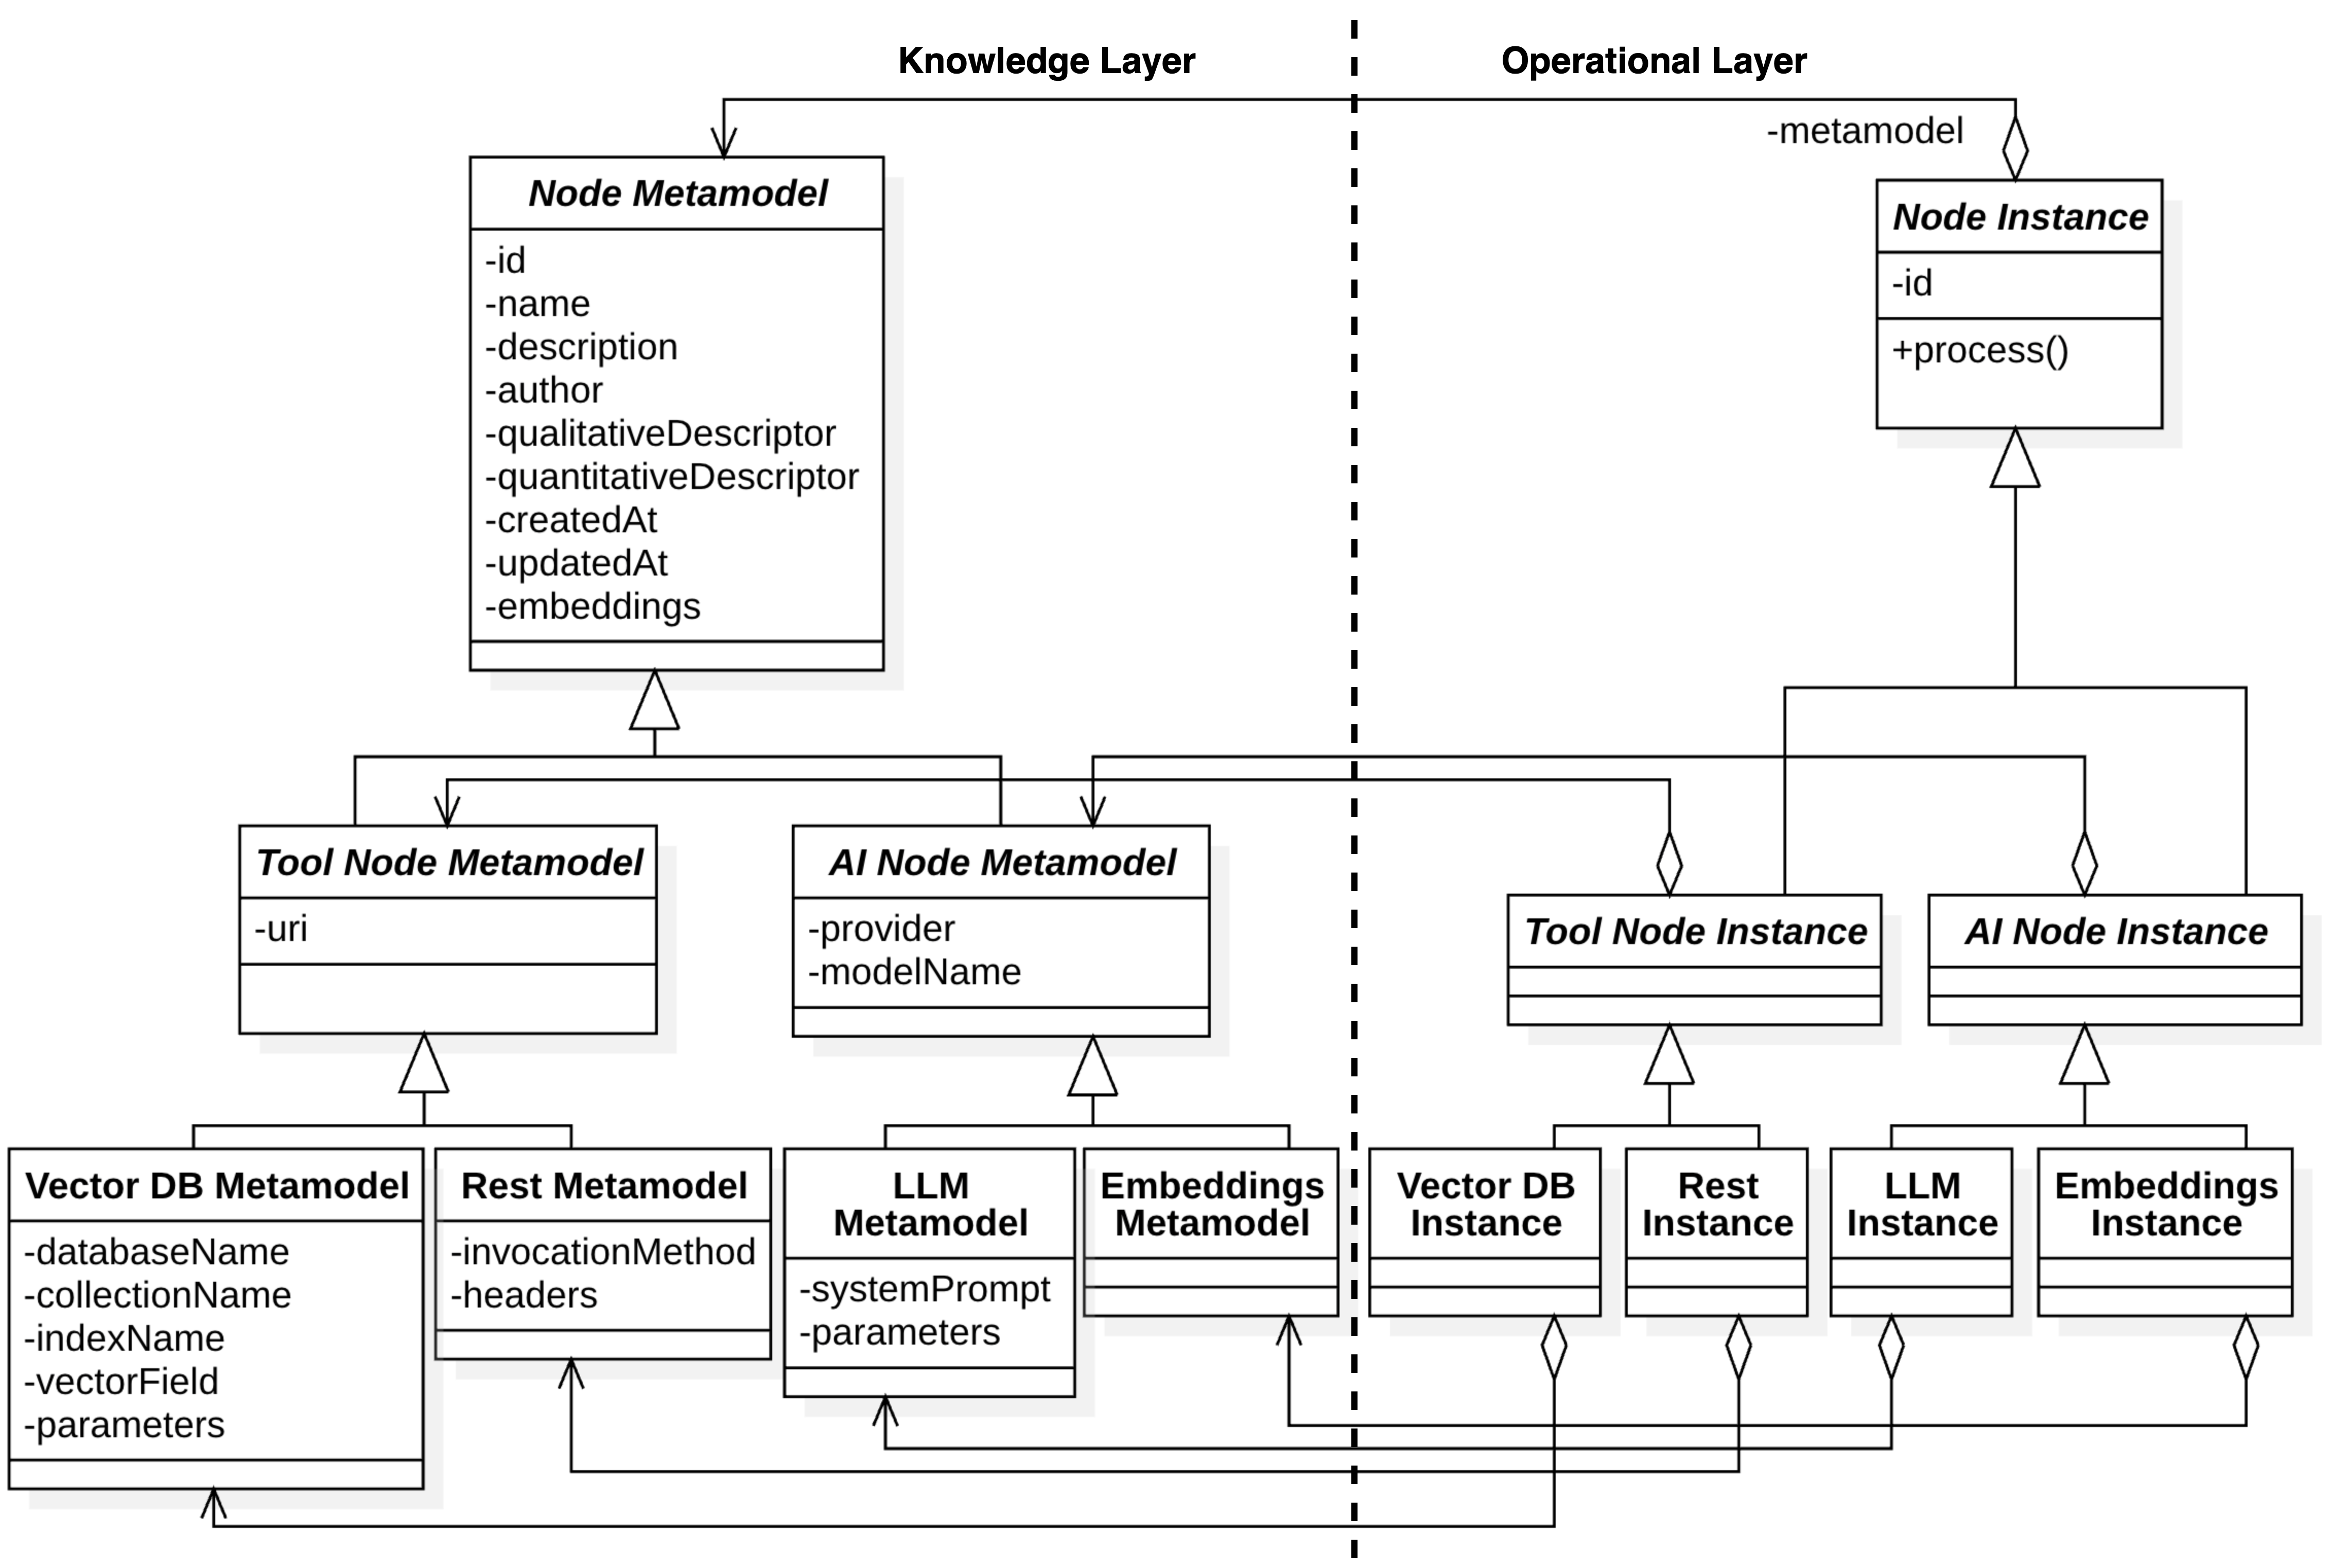
\includegraphics[width=1\textwidth]{Template_tesi/img/nodes-reflection-uml.png}
    \caption{Dual-layer architecture diagram showing Knowledge Layer meta-models (left) and their corresponding Operational Layer instances (right), illustrating the inheritance relationships between components.}
    \label{fig:nodes-reflection-uml}
\end{figure}


The nodes can be combined into workflows, which are essentially \textit{directed acyclic graphs} (DAGs). Each workflow is represented as a graph consisting of nodes and edges, where nodes correspond to specific meta-models with their associated versions, and edges define the connections between nodes within the workflow structure.
Ideally, multiple workflows can be composed together, allowing simple workflows to be reused and integrated into more complex processing pipelines. For example, the Retrieval-Augmented Generation\footnote{RAG is an AI engineering technique used to retrieve information from an external knowledge base in order to ground LLMs on accurate and up-to-date data.} (RAG) pattern can be modeled as a sub-workflow consisting of the following nodes:

\begin{enumerate}[leftmargin=*, label=\textbf{\arabic*.}]
    \item \textbf{Embedding node}: Calls an embedding model to generate a vector representation of the text input.
    \item \textbf{Vector database node}: Performs a vector similarity search against a pre-indexed data repository.
    \item \textbf{LLM node}: Receives the original query along with the retrieved documents and generates a final response.
\end{enumerate}


\begin{figure}[h]
    \centering
    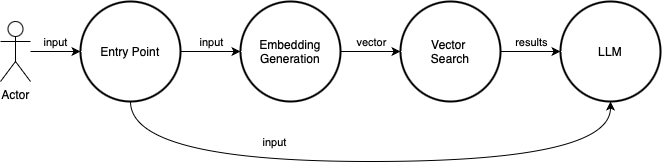
\includegraphics[width=.9\textwidth]{Template_tesi/img/RAG-workflow.png}
    \caption{Diagram of the RAG pattern workflow corresponding to the embedding, retrieval, and generation steps.}
    \label{fig:RAG-workflow}
\end{figure}










\subsubsection{Data Persistence}

A MongoDB database was selected for the meta-models repository due to its NoSQL, document-based approach. This choice is ideal for schema flexibility, especially when dealing with the evolving and heterogeneous data common in multi-agent configurations (e.g., varying parameters, node types, and data formats). Its nested structure also provides efficient storage for SBOMs. Finally, the out-of-the-box Vector Search capability provided by Atlas\footnote{\url{https://www.mongodb.com/atlas} - a fully managed Database-as-a-Service (DBaaS) provided by MongoDB.} was key in enabling semantic search for RAG, without requiring additional dedicated databases. The system uses three collections to manage:

\begin{itemize}[leftmargin=*, label=--] 
    \item The meta-models of individual nodes
    \item The meta-modes of workflows
    \item The catalog of intents handled by the system
\end{itemize}

\noindent

Although inheritance in entity modeling can add complexity to data persistence, the combination of \texttt{Jackson}’s polymorphic deserialization and \texttt{Spring Data MongoDB} effectively abstracts away this complexity. When a subclass instance is persisted, Spring automatically includes a \texttt{\_class} field in the document, which contains the fully qualified class name. This allows the framework to correctly deserialize the document and resolve the appropriate subclass during    \textit{Object-Document Mapping} (ODM).




\subsection{Structured Data Flow}


In workflow-based systems, controlling the flow of data between components is essential to ensure consistency and interoperability throughout the execution. In the context of this work, we utilize the notion of ports as an abstraction to declare the input and output interfaces of each node within the workflow. This construct promotes modular design, enables validation during data propagation, and assists in the early detection of incompatibilities. To enforce the structural correctness of meta-models, dedicated services are employed to verify the compatibility of ports across connected nodes, ensure type consistency, and validate the satisfaction of all required inputs.

\subsubsection{Input and Output Ports}

Ports act as standardized entry and exit points for data within a node.
A port is identified by a unique key and is defined by a schema that describes the expected data type and structure (e.g., primitive types, objects, arrays), supporting rich and flexible data modeling. Additionally, the port abstraction supports various specialization types which encode domain-specific semantics. For instance, in nodes representing RESTful services, ports can correspond to request body fields, query parameters, path variables, etc. In contrast, LLM-based nodes might define ports in terms of system prompt variables or user messages. An overview of the class structure used to define ports and their schema is provided in Figure~\ref{fig:port}. 


\begin{figure}[h]
    \centering
    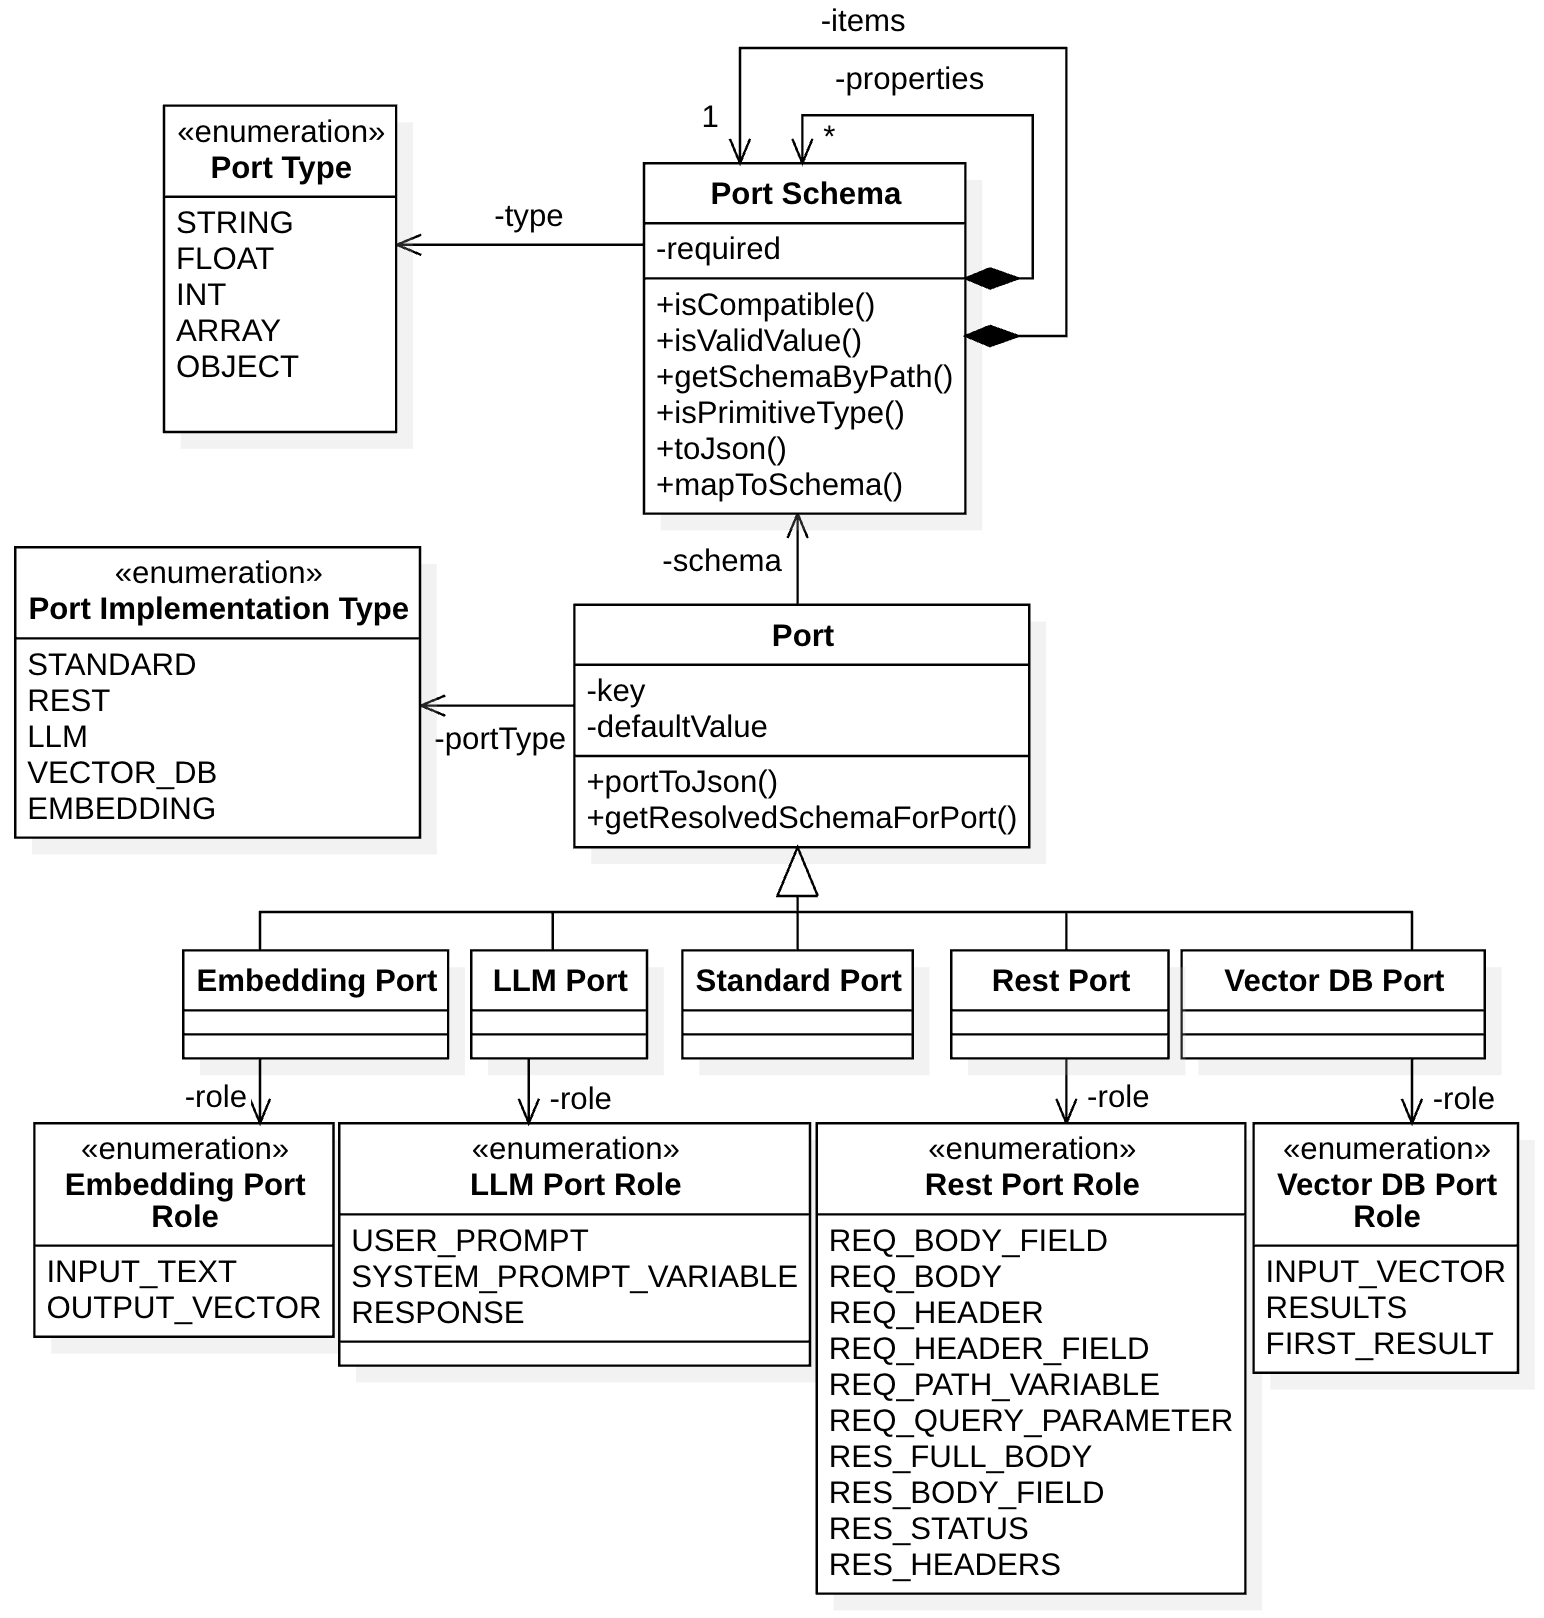
\includegraphics[width=0.8\textwidth]{Template_tesi/img/port-uml.png} 
    \caption{UML Class Diagram illustrating the \textit{Port} and \textit{Port Schema} entities, which define the structure and behavior of inputs and outputs for workflows' nodes. For brevity, the figure omits that each port implementation is associated with a corresponding builder class.
}
    \label{fig:port} 
\end{figure}



\subsubsection{LLM Structured Outputs}

When working with Large Language Models (LLMs), generating structured outputs is critical to ensure predictable consumption of the model’s responses. Spring AI addresses this need through its \textbf{Structured Output API} \cite{tzolov2024structured}, which includes a set of \textbf{Structured Output Converters}. These converters transform raw models' output into instances of predefined Java classes, leveraging prompt engineering\footnote{The process of designing inputs to effectively guide generative AI models toward desired outputs.} to guide the model's formatting behavior. Essentially, as shown in Figure~\ref{fig:structured-output-spring}, instructions are embedded in the prompts to shape the output according to the expected structure, following which the converter parses the response into a Java object.
Nevertheless, as meta-model's ports are dynamically typed and their schema is more expressive than what Spring AI supports natively, a custom converter layer was developed. This layer, built on top of the one of Spring AI,  also leverages prompt augmentation\footnote{A prompt engineering technique that enriches a base input prompt by adding context, examples, or instructions to improve the relevance, accuracy, or specificity of the AI's response.} to map the LLM responses to the corresponding output port schema declared in the meta-model.

\begin{figure}[H]
    \centering
    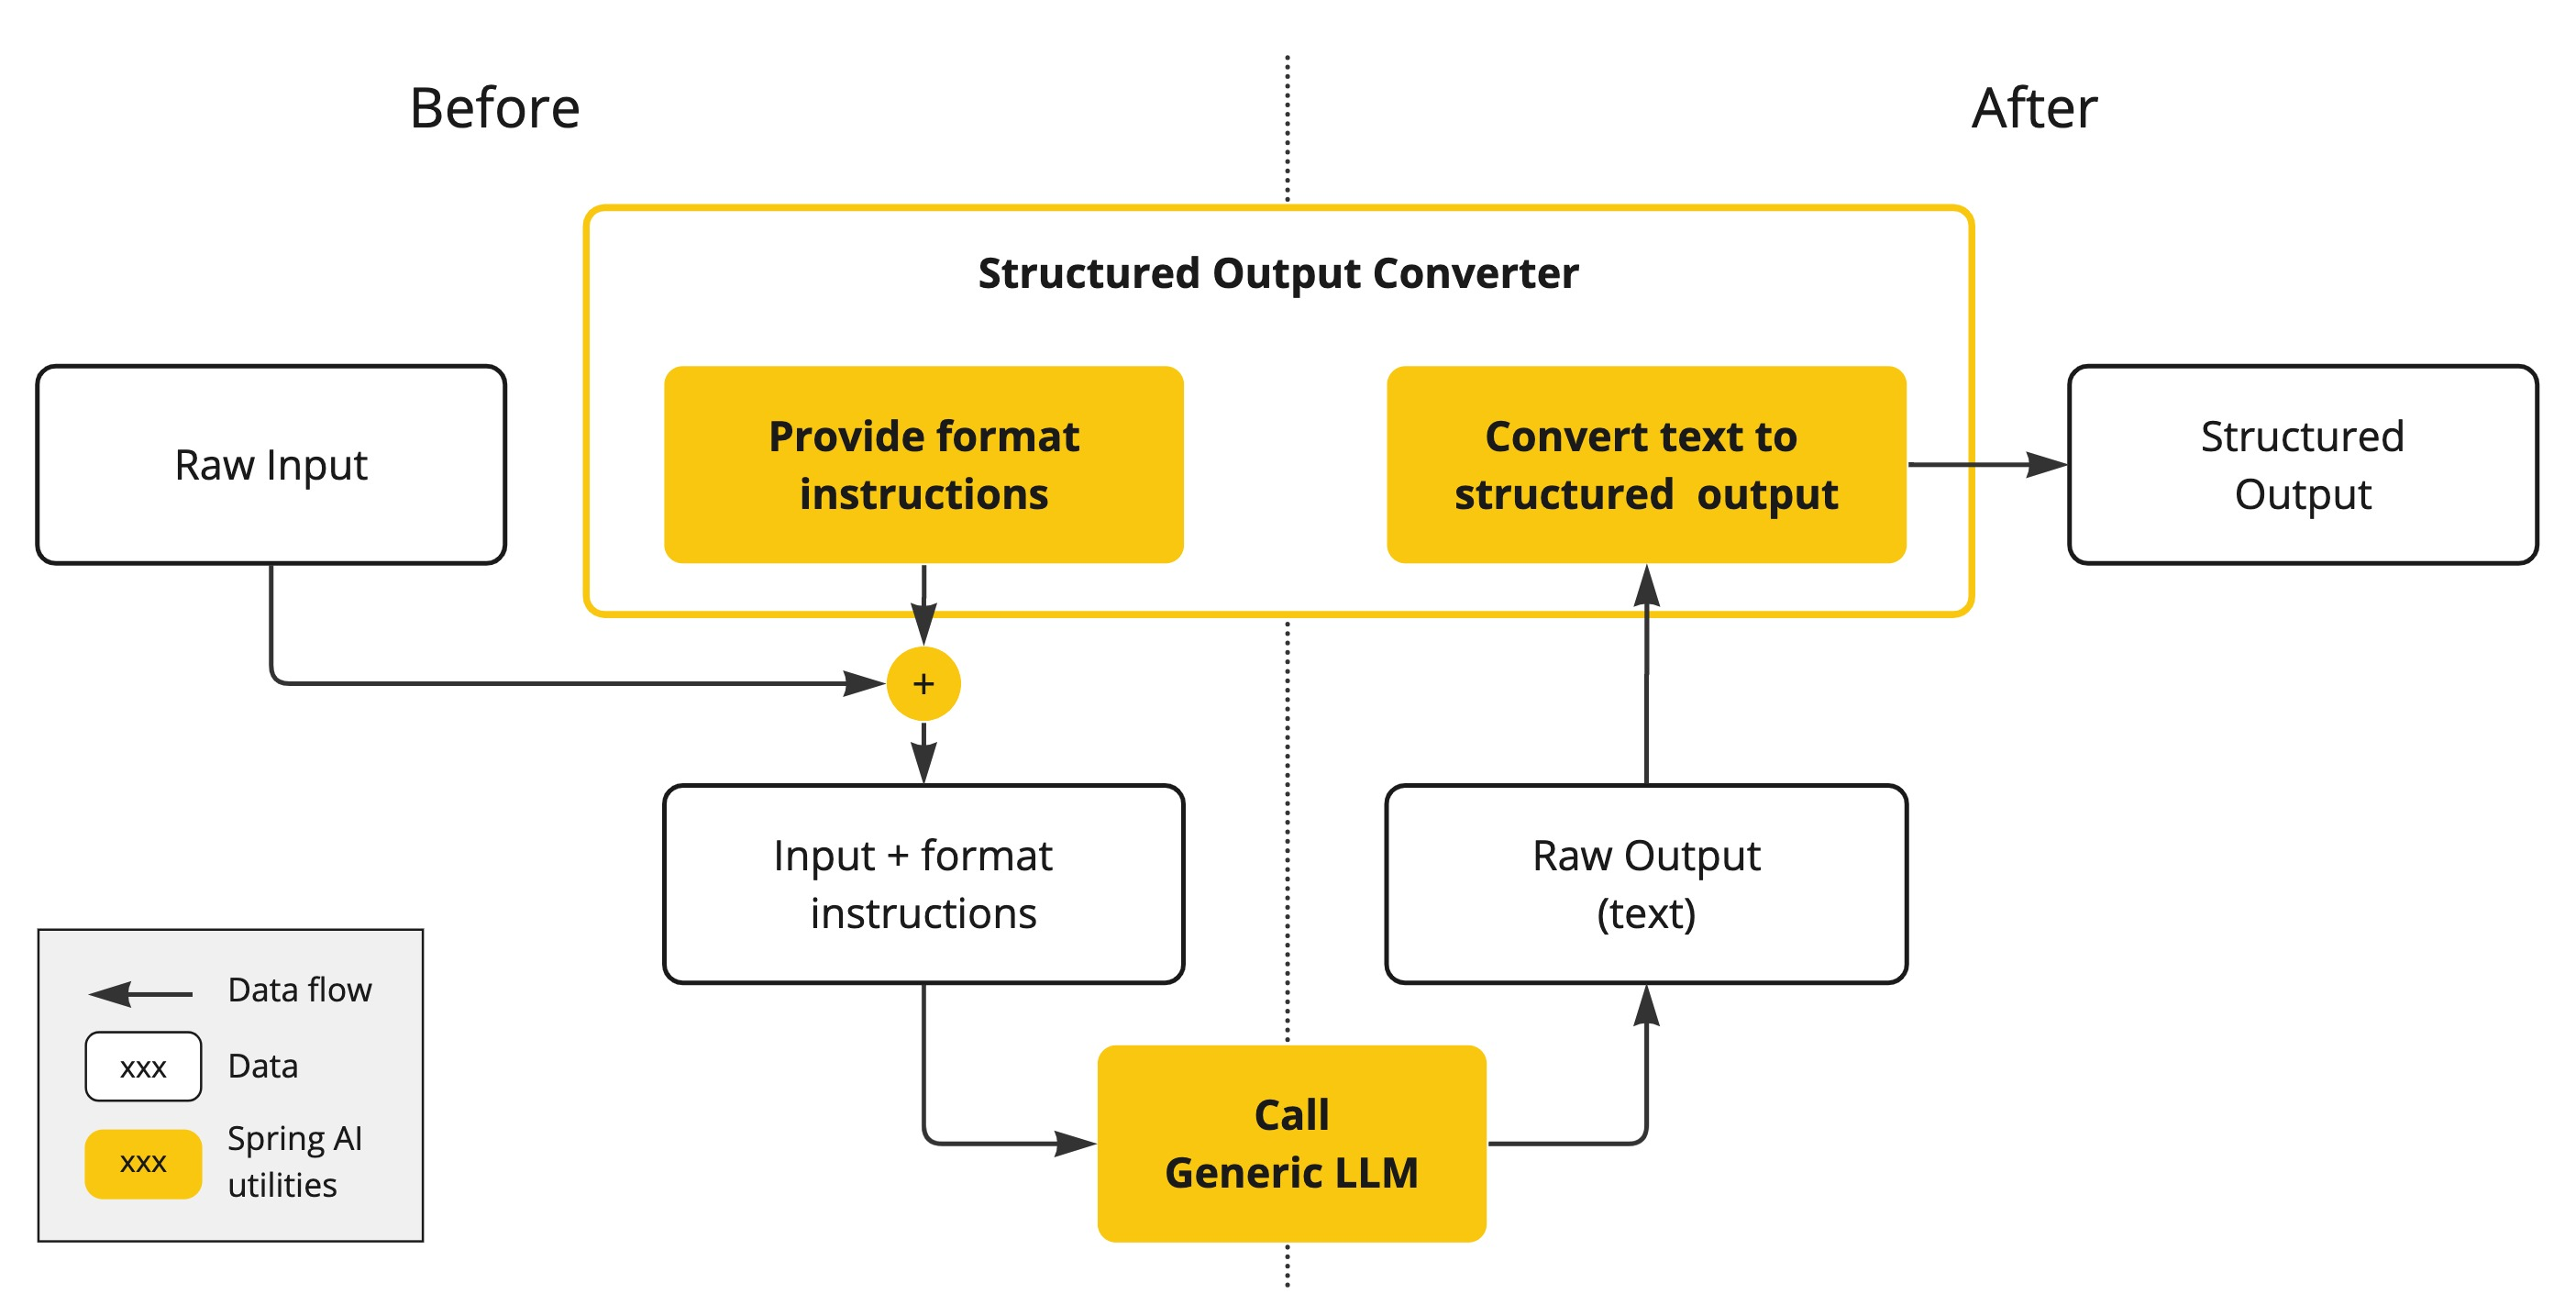
\includegraphics[width=1\textwidth]{Template_tesi/img/structured-output.jpg}
    \caption{Overview of Spring AI's Structured Output Converters. From \url{https://spring.io/blog/2024/05/09/spring-ai-structured-output}}
    \label{fig:structured-output-spring} 
\end{figure}




\subsubsection{Edge Bindings} \label{sec:bindings}
A central concept to facilitate the collaboration of nodes within workflows is the idea of bindings. These specify how the output of one node connects to the input of the following node. This is particularly important in heterogeneous systems where different nodes might use different naming conventions or data formats for interface ports. Bindings operate in two modes:

\begin{itemize}[leftmargin=*, label=--]
    \item \textbf{Explicit Bindings}: These are direct mappings between input and output port names. As aliases, they allow ports with different names to be connected explicitly.
    \item \textbf{Implicit Matching}: When no bindings are provided, the system attempts to connect ports with the same key name, assuming their schema is compatible. 
\end{itemize}


This mechanism is essential for enabling interoperability between components provided by different vendors or when combining general-purpose nodes with more specialized ones. Importantly, while bindings can be manually defined at design time, they can also be determined dynamically at runtime through the use of an LLM-based agent. In our implementation, this agent is referred to as the \texttt{Port Adapter Service}, which enables the adaptiveness of the system. The service takes as input the schemas of two port sets—source and target—and generates a bindings map by matching fields based on names, types, structure, and required fields. It supports nested objects through dot notation\footnote{Dot notation is a syntax used to access nested fields in structured data (e.g., \texttt{user.address.city}), commonly found in formats like JSON or object schemas.} and applies renaming where needed to ensure schema alignment.




\subsection{Workflow Execution} \label{sec:execution}

For the purposes of this project, the workflow engine was built entirely from the ground up, despite considering alternatives like \textit{n8n}\footnote{
n8n is a workflow automation tool. See \url{https://n8n.io/}}.
While the Operational Layer is the core of the system—where the actual execution of workflows takes place—it heavily relies on the Knowledge Layer. As shown in Figure \ref{fig:exec}, the Knowledge Layer is accessed through the \textit{MOP} (Meta Object Protocol), as already introduced in Section \ref{sec:reflection}. The MOP encapsulates meta-model services that directly interface with the three repositories: Metamodel Catalogs of Workflow, Nodes, and Intents. Therefore, the MOP acts as the controller of meta-models and provides the only possible way for the Operational Layer to fetch and update them. Additionally, it handles event dispatching and, through dedicated services such as the \texttt{Workflow Metamodel Validator} and \texttt{Node Metamodel Validator}, ensures the structural integrity of these meta-objects. The complete execution process proceeds as follows:

\begin{enumerate}[leftmargin=*, label=\textbf{\arabic*.}]
    \item\textbf{Intent Detection}: \texttt{The Intent Detection Service} identifies the user's intent from natural language input. It retrieves relevant intents from the Knowledge Layer for RAG and extracts unstructured variables. If no matching intent exists, it creates a new one with associated metadata.
    \item\textbf{Workflow Selection}:  The \texttt{Routing Manager} selects a workflow corresponding to the detected intent by querying available workflows. If multiple matches are found, selection can be guided by intent-specific scores—derived from user feedback, comparative evaluation, or an \textit{AI judge}\footnote{An AI model that is used to evaluate the output of other AI systems \cite{huyen2024ai}}—while a temperature-based sampler ensures diversity in the final choice.
    \item\textbf{Workflow Retrieval}: The \texttt{Workflow Instance Manager} retrieves an existing workflow from the registry or instantiates a new one if none exists by fetching up-to-date information from the Knowledge Layer.
    \item\textbf{Workflow Execution}: The \texttt{Input Mapper Service} (LLM-powered) binds the extracted input data to the entry ports of the workflow. The \texttt{Workflow Executor} then runs the process, supported by the \texttt{Port Adapter Service} (LLM-powered), which resolves any port mismatches experienced during execution.
\end{enumerate}


\begin{figure}
  \centering
  \begin{adjustbox}{center}
    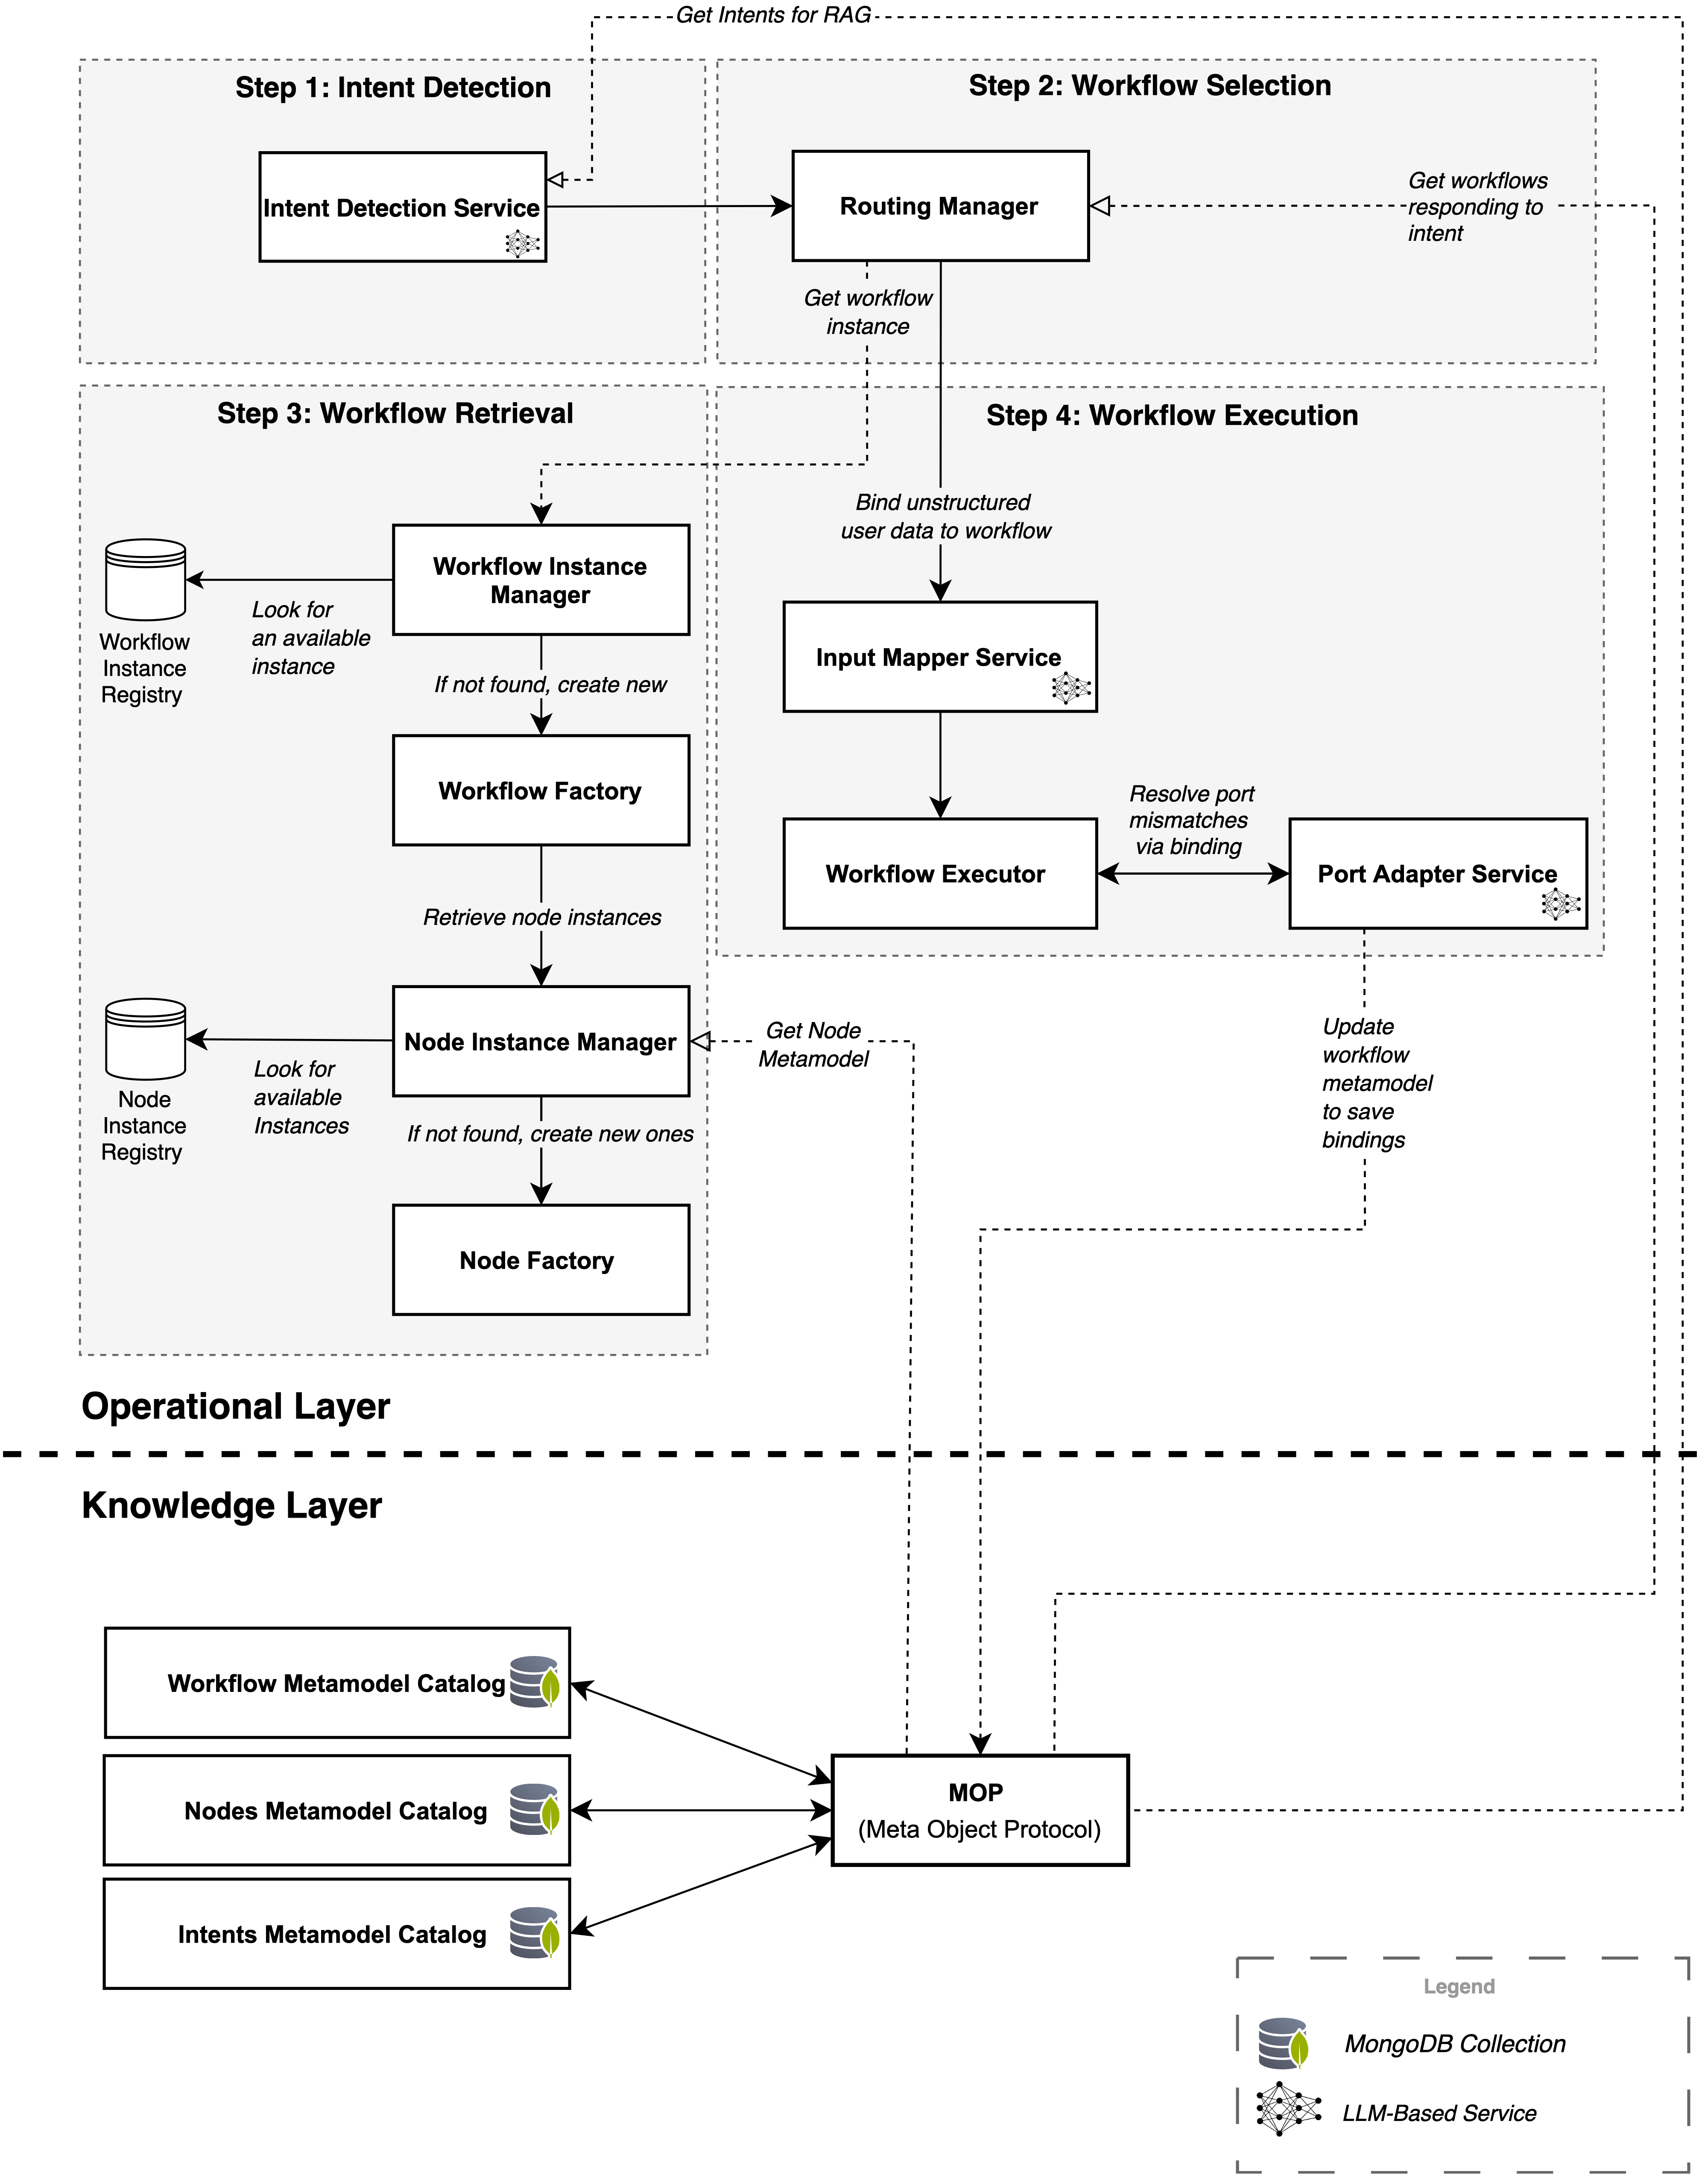
\includegraphics[width=1.2\textwidth]{Template_tesi/img/execution.png}
  \end{adjustbox}
  \caption{Workflow Execution four-step process, showing the interaction between the Operational Layer components and the Knowledge Layer accessed through the MOP and its three meta-model catalogs.}
  \label{fig:exec}
\end{figure}


\subsubsection{Ports Adaption}

As previously mentioned, the \texttt{Port Adapter Service} is essential for ensuring system adaptability and the interoperability of components, even when these components are developed independently or by third-party vendors. Since nodes are not necessarily aware of each other, aligning components with mismatched input and output interfaces is critical to achieving component reusability.
As discussed in Section \ref{sec:bindings}, edge bindings between components can be resolved at runtime. This task is handled by the \texttt{Port Adapter Service}, which is triggered by the \texttt{Workflow Executor} whenever a node about to be executed lacks the necessary input data in the current execution context. If a functional adaptation is found, the Operational Layer interacts with the Knowledge Layer to update the workflow meta-model. As a result, following executions of the same workflow will skip the adaptation step, reducing execution time. Figure \ref{fig:adaption-flow-chart} provides a summary of this dynamic adaptation process.
Ultimately, this mechanism significantly improves the \textbf{resilience of the system}: when a workflow depends on a node whose interface changes (e.g., due to a breaking change), the system can attempt to automatically resolve any incompatibilities introduced by that change.

\begin{figure}[h]
    \centering
    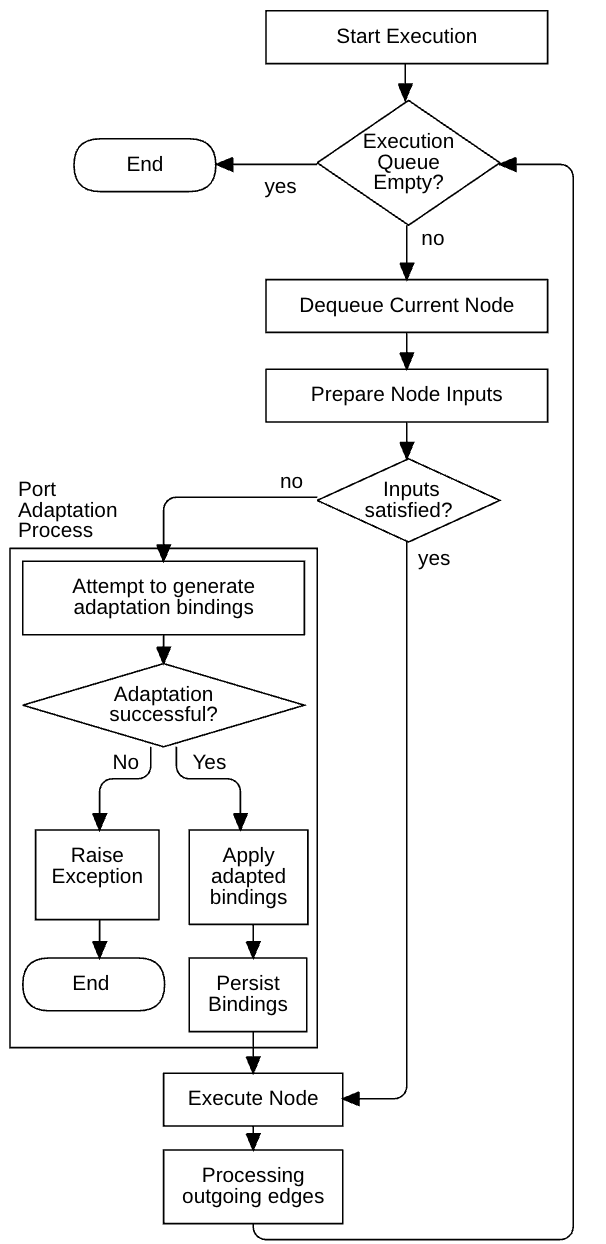
\includegraphics[width=.45\textwidth]{Template_tesi/img/adaption.png}
    \caption{Flowchart of the workflow nodes execution process, detailing the dynamic port adaptation process.}
    \label{fig:adaption-flow-chart} 
\end{figure}


\subsubsection{Workflow Synthesis}


The true potential of this architecture and the SBOM becomes apparent when during the \textit{Workflow Retrieval} phase (Step 3) no pre-assembled workflow capable of handling the user’s intent is found in the Knowledge Base. In such cases, the system can leverage \textit{SBOM-like information} in the Knowledge Layer, which becomes central to the process. This enables the dynamic construction of new workflows by intelligently combining existing nodes. 

Each node is associated with both qualitative and quantitative descriptors—structured and unstructured—which describe its functionality and specifications. These descriptors are embedded and indexed to support \textbf{Hybrid Search}\footnote{An information retrieval method that combines semantic search with full-text search, merging results using algorithms such as Reciprocal Rank Fusion to improve relevance.}, allowing an LLM agent to retrieve and compose components based on their declared capabilities.

This mechanism enables the system to generate workflows that meet \textbf{previously unanticipated requirements}. For instance, if the intent introduces a new constraint, such as a specific latency threshold, the system can construct a workflow by including only nodes whose descriptors indicate compatibility with that latency requirement. Similarly, this applies to verifying the legal compliance or certification status of nodes and tools. Moreover, this mechanism fosters interoperability between vendors, overcoming the major challenges related to the \textbf{lack of standardization} in SBOMs and AIBOMs. Even without a shared or predefined standard or grammar for tracking node dependencies and specifications, considering that different providers may disclose only partial data or use varying formats, an AI-driven approach can transcend these limitations.





Once a suitable workflow is synthesized, it can be saved in the Knowledge Base for future retrieval and reuse. New workflows can be evaluated using established methods such as AI-based judgment, human evaluation, or \textbf{consensus-based voting}. In the latter, multiple agents specialized in workflow construction independently generate candidate workflows, and a workflow is accepted only if it is produced by a majority of agents.

While this high-level approach is promising and underscores the importance of the meta-model repository, further research is required to formalize and systematically structure the process of automatic workflow synthesis.












\subsection{Runtime Adaptations}

As previously discussed, a central advantage of the Reflection pattern is its support for runtime adaptability. In the proposed architecture, agents both retrieve and modify knowledge during execution to accommodate modifications in the environment, dependency structures, or evolving user requirements.
Operational agents interact with the Knowledge Layer to query or update system knowledge in response to runtime conditions. These updates may originate \textbf{externally}—such as from software releases, dependency upgrades, or the introduction of new meta-models—or be \textbf{triggered internally} by components (e.g., the \texttt{Port Adapter Service}; see Section \ref{sec:bindings}) or by system processes (e.g., the generation of new intents and workflows; see \textit{Workflow Execution}, Section \ref{sec:execution}).
To ensure synchronization and consistency between the operational level and the Knowledge Layer, meta-model changes are propagated as events. These events, dispatched via the Meta-Object Protocol (MOP), are received by subscribed operational components, which then adapt their configurations accordingly (see Figure \ref{fig:node-update-event}).


\begin{figure}[h]
    \centering
    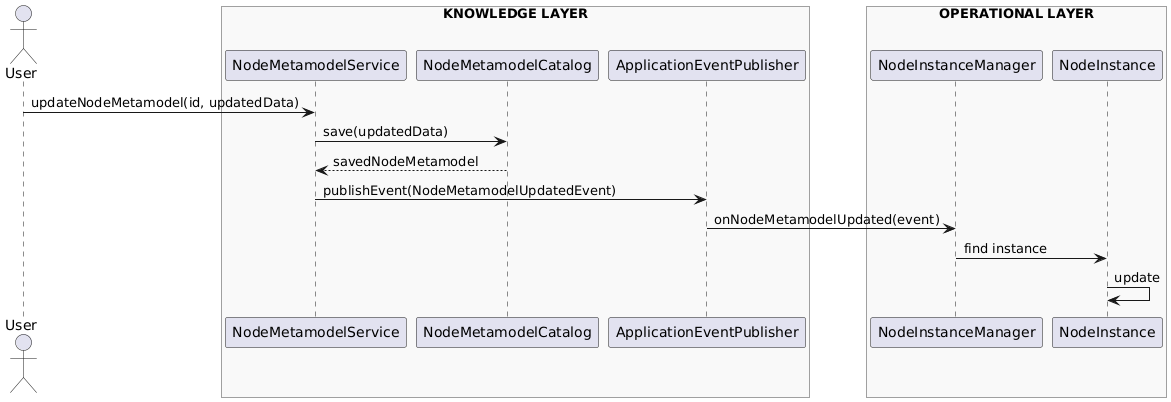
\includegraphics[width=1\textwidth]{Template_tesi/img/node-update-event.png}
    \caption{Propagation of meta-model updates from the Knowledge Layer to operational components via the MOP.}
    \label{fig:node-update-event} 
\end{figure}


\subsubsection{Meta-models Versioning}
In the proposed implementation, the versioning of meta-model catalogs follows the Semantic Versioning\footnote{A versioning scheme that uses the format \texttt{MAJOR.MINOR.PATCH} to indicate the type and impact of changes.} standard.


\begin{itemize}[leftmargin=*, label=--] 
    \item Minor and patch version changes are applied in place within the existing document.
    \item Major version changes (i.e., breaking updates) result in the creation of a new meta-model entry within the catalog.

\end{itemize}



\noindent
Therefore, each meta-model is identified by a unique ID and a family ID, which groups all versions belonging to the same logical component. Within a workflow, nodes reference a specific version of a node.






\subsubsection{Strategies for Instance Updates}
Two primary operational update strategies are employed depending on the nature of the meta-model change:


\begin{itemize}[leftmargin=*, label=--] 
    \item \textbf{Hot-Swapping}: For non-breaking updates, if the instance is not currently running, the system may swap the meta-model in place, seamlessly refreshing the instance.
    \item \textbf{Re-instantiation}: In cases where the instance is currently active or the update constitutes a breaking change (e.g., altered node dependencies in a workflow), the affected meta-model is marked as deprecated. Any future execution of such instances requires a complete re-creation, even if it was previously persisted in the registry.
\end{itemize}







